\section{Aprendizado de Máquina}

Esta seção dedica-se à apresentação dos fundamentos conceituais e matemáticos do Aprendizado de Máquina, com ênfase nas abordagens supervisionadas e profundas aplicadas à análise de sinais. Inicialmente, discorrem-se os paradigmas de aprendizado, os principais algoritmos utilizados e suas respectivas áreas de aplicação. Em seguida, introduz-se o Aprendizado Profundo, e as Redes Neurais Multicamada Unidimensionais, destacando seu papel na extração automática de padrões complexos em sinais acústicos, como os gerados por fenômenos de cavitação e falhas incipientes em equipamentos rotativos.

A Inteligência Artificial constitui um campo interdisciplinar dedicado ao desenvolvimento de sistemas computacionais capazes de executar tarefas tradicionalmente associadas à cognição humana, tais como percepção, reconhecimento de padrões, tomada de decisão e raciocínio adaptativo. Seu objetivo central é reproduzir — e, em algumas situações, superar — aspectos do comportamento inteligente por meio de modelos matemáticos, estruturas algorítmicas e processamento de grandes volumes de dados.

Dentro desse panorama, o Aprendizado de Máquina representa uma subárea fundamental, responsável pelo estudo de algoritmos que aprendem a partir de exemplos. Em vez de depender de regras fixas programadas manualmente, esses algoritmos ajustam seus parâmetros internos de forma automática quando expostos a novos dados, aprimorando progressivamente seu desempenho em tarefas específicas. Essa característica torna o AM particularmente adequado a problemas complexos, não lineares ou de natureza estocástica, nos quais abordagens analíticas \mbox{tradicionais apresentam limitações.}

Entre os métodos mais influentes de Aprendizado de Máquina destacam-se as Redes Neurais Artificiais, inicialmente inspiradas em princípios do processamento neural biológico, desde o modelo formal de neurônio proposto por \citeonline{mcculloch1943logical} até as formulações consolidadas em obras clássicas como \citeonline{haykin2001redes}. Embora tais modelos tenham se tornado a base das arquiteturas modernas de aprendizado profundo, eles representam abstrações significativamente simplificadas do funcionamento do sistema nervoso real, empregando ativações contínuas e sincronizadas que não refletem diretamente a natureza pulsada e esparsa da comunicação neuronal biológica.

%Estudos recentes, como o de \citeonline{zheng2022introductory}, ampliam essa discussão ao comparar as Redes Neurais Artificiais convencionais (\textit{Artificial Neural Networks, ANNs}) com as Redes Neurais Pulsadas (\textit{Spiking Neural Networks, SNNs)}, modelos que buscam aproximar de forma mais fidedigna a dinâmica eletrofisiológica observada em neurônios reais. Enquanto as ANNs utilizam funções de ativação contínuas e densas, as SNNs operam com eventos discretos de disparo, \textit{spikes}, permitindo codificação temporal, maior esparsidade e potencial redução significativa no consumo energético. Além disso, diferem quanto aos mecanismos de aprendizagem: ao passo que as ANNs dependem tipicamente do \textit{backpropagation} e de gradientes contínuos, as SNNs investigam regras de aprendizado local inspiradas na biologia, como o \mbox{\textit{Spike-Timing-Dependent Plasticity, STDP.}}
%
%Assim, a literatura contemporânea evidencia uma evolução no entendimento da relação entre modelos computacionais e sistemas biológicos: as ANNs permanecem essenciais para aplicações práticas em larga escala devido à maturidade de suas técnicas de otimização, enquanto as SNNs representam uma fronteira promissora rumo a arquiteturas mais eficientes, esparsas e biologicamente plausíveis, conectando de modo mais direto os princípios da inteligência natural aos mecanismos da inteligência artificial.
%
%Nas redes naturais, cada neurônio, Figura \ref{fig:neuronio} é constituído por dendritos (responsáveis pela recepção dos estímulos provenientes de outras células), pelo corpo celular (que integra e processa os sinais recebidos) e pelo axônio (que transmite a saída para outras células). A comunicação ocorre por meio de impulsos elétricos, cuja frequência determina o nível de ativação do neurônio \citeonline{haykin2001redes}. Ainda que as redes biológicas não transmitam sinais negativos e apresentem organização morfológica extremamente heterogênea, constituem o modelo conceitual que fundamenta a criação das RNAs.
%
%\begin{figure}[H]
%	\centering
%	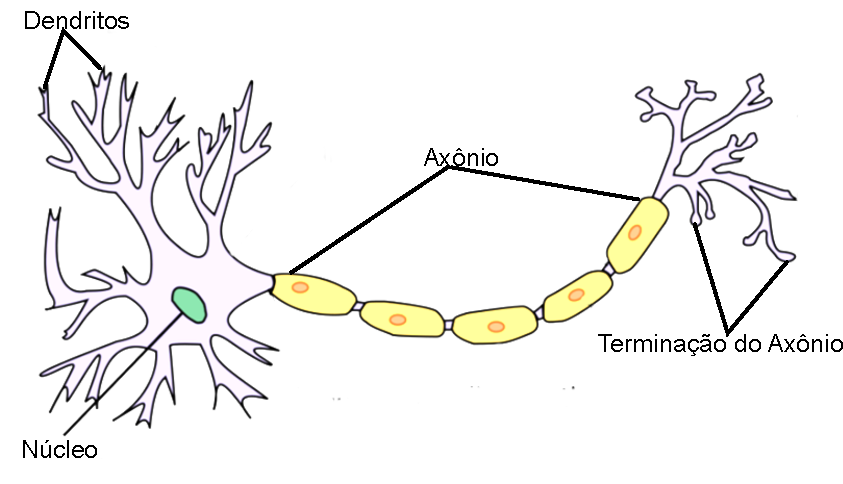
\includegraphics[width=0.65\linewidth]{figs/AprendizadoDeMaquina/Neuronio}
%	\caption{Ilustração de um Neurônio. Adaptado de \citeonline{zheng2022introductory}.}
%	\label{fig:neuronio}
%\end{figure}
%
%O neurônio artificial, por sua vez, é uma abstração computacional que captura os elementos essenciais do processo biológico:
%\begin{enumerate}[label=(\roman*)]
%	\item entradas provenientes do meio ou de outros neurônios;
%	\item sinapses simuladas por pesos, $w_1, w_2, w_3, ... w_n$ que modulam a influência de cada entrada;
%	\item um termo de viés (bias), que desloca a função de ativação e permite maior flexibilidade ao modelo;
%	\item um somador, responsável por combinar as entradas ponderadas;
%	\item uma função de ativação, que limita ou transforma a amplitude do sinal gerado; e
%	\item uma saída, transmitida à próxima camada da rede.
%\end{enumerate}
%
%Em conjunto, múltiplos neurônios artificiais organizados em camadas interconectadas formam arquiteturas capazes de aproximar funções complexas, detectar regularidades em dados ruidosos e extrair características relevantes de sinais multidimensionais. Essa capacidade emergente explica o amplo uso das RNAs em visão computacional, processamento de sinais, reconhecimento de fala, análise temporal e, particularmente neste trabalho, detecção de padrões em sinais de Emissão Acústica.
%
%\begin{figure}[H]
%	\centering
%	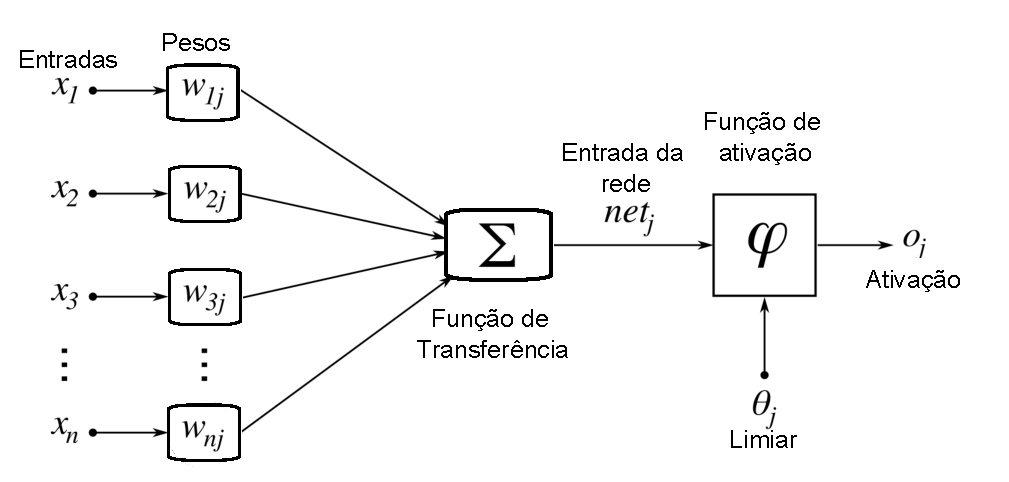
\includegraphics[width=0.85\linewidth]{figs/AprendizadoDeMaquina/NeuronioArtificial}
%	\caption{Neurônio artificial. Fonte: O autor.}
%	\label{fig:artificialneuronmodelenglish}
%\end{figure}
%
%O processo de aprendizado pode ocorrer de diferentes formas, dependendo da disponibilidade e do tipo de informação fornecida ao modelo. De modo geral, o ML é classificado em três categorias principais: aprendizado supervisionado, em que o modelo é treinado com exemplos rotulados; aprendizado não supervisionado, no qual se busca identificar padrões e agrupamentos ocultos em dados não rotulados; e aprendizado por reforço, baseado na interação contínua de um agente com um ambiente para maximizar recompensas acumuladas. Cada uma dessas abordagens apresenta características próprias e é adequada a contextos específicos de aplicação, como classificação, regressão, agrupamento e controle adaptativo.

Um subconjunto mais avançado e especializado do ML é o Aprendizado Profundo, que emprega arquiteturas compostas por múltiplas camadas de processamento, as chamadas redes neurais profundas. Essas estruturas são inspiradas no funcionamento do cérebro humano e são capazes de extrair representações hierárquicas e abstratas dos dados, capturando padrões complexos e não lineares. O DL tem se destacado em aplicações de alto impacto, como reconhecimento de voz e imagem, tradução automática, diagnóstico médico assistido e análise de sinais dinâmicos, devido à sua notável capacidade de generalização e robustez frente a grandes volumes de informação.

Nos últimos anos, a combinação entre aprendizado profundo e dispositivos de alto desempenho, como GPUs e FPGAs, tem ampliado significativamente o escopo de aplicação dessas técnicas, tornando viável a análise em tempo real de dados de alta taxa de amostragem — como os provenientes de sensores acústicos e vibrométricos empregados no monitoramento de máquinas rotativas. Essa integração entre IA e instrumentação digital representa um dos pilares do paradigma da manutenção preditiva inteligente, na qual modelos treinados são utilizados para detectar anomalias, prever falhas e otimizar a operação de sistemas industriais complexos.

%
%O campo do aprendizado de máquina abrange diferentes abordagens de treinamento, cada uma fundamentada na forma como o modelo interage com os dados e aprende a partir deles. De maneira geral, essas abordagens são organizadas em três grandes paradigmas: o aprendizado supervisionado, o aprendizado não supervisionado e o aprendizado por reforço. Cada paradigma apresenta características próprias, vantagens e limitações, sendo aplicável a diferentes tipos de problemas de modelagem, classificação e \mbox{controle em sistemas complexos.}

Os três paradigmas são sistematizados na Figura~\ref{fig:AprendizadoDeMaquinaConceitos}, que apresenta uma visão comparativa das principais estratégias de aprendizado e suas aplicações típicas em contextos industriais. Cada paradigma difere quanto à forma de aprendizado, à disponibilidade de rótulos nos dados e ao tipo de \textit{feedback} recebido durante o processo de treinamento.

\begin{figure}[H]
    \centering
    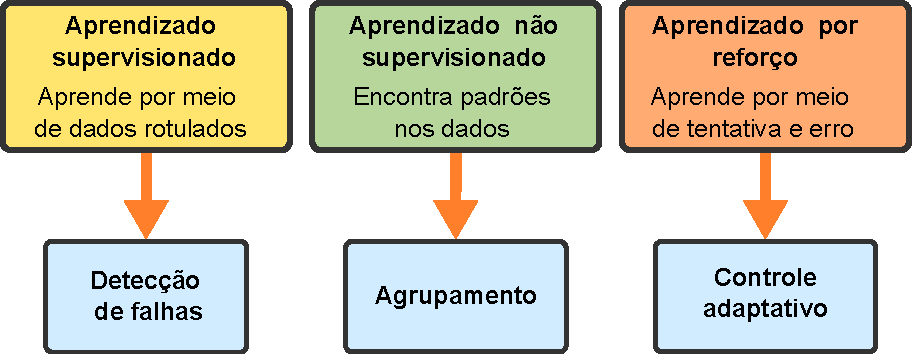
\includegraphics[width=0.7\linewidth]{figs/AprendizadoDeMaquina/AprendizadoDeMaquinaConceitos.pdf}
    \caption{Paradigmas do aprendizado de máquina e exemplos de aplicação industrial.\\Fonte: Em destaque o paradigma utilizado neste trabalha. O autor.}
    \label{fig:AprendizadoDeMaquinaConceitos}
\end{figure}

\begin{itemize}
    \item \textbf{Aprendizado Supervisionado:} Baseia-se na utilização de conjuntos de dados rotulados, nos quais cada amostra possui uma resposta conhecida. O modelo é treinado para aprender a relação entre entradas e saídas, generalizando o comportamento para novos dados. É amplamente empregado em tarefas de classificação e regressão, como a \textbf{detecção de falhas em sensores} ou a previsão de desgaste de componentes em bombas e turbinas.

    \item \textbf{Aprendizado Não Supervisionado:} Opera sobre dados não rotulados, buscando identificar padrões e estruturas ocultas. Utiliza técnicas como o \textit{k-means} ou análise de componentes principais (PCA) para agrupar dados semelhantes ou reduzir dimensionalidade. Essa abordagem é especialmente útil para \textbf{agrupamento de modos de operação}, detecção de anomalias e análise exploratória de sinais industriais.

    \item \textbf{Aprendizado por Reforço:} Difere dos paradigmas anteriores por envolver a interação contínua entre um agente e um ambiente. A cada ação, o agente recebe uma recompensa ou penalidade, aprendendo a maximizar seu desempenho ao longo do tempo. Esse método é aplicado em \textbf{controle adaptativo de processos industriais}, robótica e otimização de sistemas dinâmicos sob condições variáveis.
\end{itemize}

A Figura~\ref{fig:AprendizadoDeMaquinaConceitos} sintetiza graficamente essa classificação, destacando a complementaridade entre os paradigmas de Aprendizado Supervisionado, Não Supervisionado e por Reforço. Essa taxonomia ressalta a relevância das técnicas de \textit{Machine Learning} para a construção de sistemas inteligentes que não apenas identificam falhas, mas extraem conhecimento útil para otimizar processos. Em última análise, o diagrama ilustra o arcabouço conceitual para o desenvolvimento de soluções voltadas à manutenção preditiva, à análise de falhas em componentes mecânicos e ao monitoramento em  com baixa latência de inferência, promovendo a detecção precoce de anomalias e garantindo a maior robustez de decisão no ambiente industrial.

%O aprendizado de máquina engloba uma ampla variedade de algoritmos, cada um com princípios matemáticos e áreas de aplicação específicas. A escolha do modelo mais adequado depende diretamente da natureza dos dados, do objetivo da análise e das restrições computacionais do sistema. De forma geral, entre os principais algoritmos utilizados em ML, são:
%
% \begin{itemize}
%     \item \textbf{Redes Neurais Artificiais (ANNs):} inspiradas no funcionamento biológico do cérebro, compostas por camadas de neurônios interconectados capazes de aprender relações complexas entre variáveis.
%     \item \textbf{Árvores de Decisão e Random Forest:} modelos baseados em regras hierárquicas que realizam divisões sucessivas do espaço de dados, amplamente empregados em classificação e regressão devido à sua interpretabilidade.
%     \item \textbf{Máquinas de Vetores de Suporte (SVMs):} algoritmos que buscam maximizar a margem entre classes, eficazes em conjuntos de dados de alta dimensionalidade e com fronteiras não lineares.
%     \item \textbf{Modelos de Mistura Gaussiana (GMMs):} utilizados para modelar distribuições probabilísticas complexas e realizar agrupamento (clustering) de dados de natureza heterogênea.
%     \item \textbf{Métodos de Ensemble, como Gradient Boosting:} combinam múltiplos modelos fracos (geralmente árvores de decisão) para formar um modelo forte, otimizando o desempenho preditivo e reduzindo o erro de generalização.
%     \item \textbf{Redes Neurais Multicamada (MLP):} arquiteturas profundas projetadas para extrair automaticamente padrões espaciais ou temporais, amplamente empregadas em visão computacional, processamento de áudio e diagnóstico industrial.
% \end{itemize}

%\begin{table}[H]
%\centering
%\caption{Principais algoritmos de aprendizado de máquina e suas características gerais.}
%\label{tab:algoritmos_ml}
%\renewcommand{\arraystretch}{1.3}
%\resizebox{\textwidth}{!}{%
%\begin{tabular}{p{4cm} p{11cm}}
%\hline
%\textbf{Algoritmo} & \textbf{Descrição Geral} \\ \hline
%
%\textbf{Redes Neurais Artificiais (ANNs)} &
%Inspiradas no funcionamento biológico do cérebro, são compostas por camadas de neurônios interconectados capazes de aprender relações complexas entre variáveis, sendo adequadas para modelar fenômenos não lineares. \\ \hline
%
%\textbf{Árvores de Decisão e Random Forest} &
%Modelos baseados em regras hierárquicas que realizam divisões sucessivas do espaço de dados. São amplamente empregados em tarefas de classificação e regressão, destacando-se pela interpretabilidade e robustez a ruído. \\ \hline
%
%\textbf{Máquinas de Vetores de Suporte (SVMs)} &
%Algoritmos que buscam maximizar a margem entre classes, sendo eficazes em conjuntos de dados de alta dimensionalidade e com fronteiras não lineares, especialmente em classificações binárias. \\ \hline
%
%\textbf{Modelos de Mistura Gaussiana (GMMs)} &
%Utilizados para modelar distribuições probabilísticas complexas, permitindo identificar grupos latentes de dados (\textit{clustering}) em aplicações de natureza heterogênea e não supervisionada. \\ \hline
%
%\textbf{Métodos de Ensemble (ex.: Gradient Boosting)} &
%Combinam múltiplos modelos fracos (geralmente árvores de decisão) para formar um modelo mais robusto, otimizando o desempenho preditivo e reduzindo o erro de generalização. \\ \hline
%
%\textbf{Redes Neurais Multicamada (MLP)} &
%Arquiteturas profundas projetadas para extrair automaticamente padrões espaciais ou temporais por meio de filtros convolucionais, amplamente aplicadas em visão computacional, processamento de sinais acústicos e diagnóstico industrial. \\ \hline
%\end{tabular}}
%\end{table}
%
%Entre esses métodos, as \textbf{Redes Neurais Multicamada (MLP)} merecem destaque por sua capacidade de extrair representações hierárquicas de dados brutos, reduzindo a necessidade de pré-processamento manual. Embora originalmente concebidas para o reconhecimento de imagens, as MLP têm-se mostrado extremamente eficazes na análise de sinais acústicos e séries temporais, como os provenientes de sensores de emissão acústica, devido à sua habilidade em capturar correlações locais \mbox{e padrões de alta frequência.}
%
%A arquitetura típica de uma CNN é composta por diferentes tipos de camadas, cada uma com função específica no processo de aprendizado:
%
%\begin{itemize}
%    \item \textbf{Camadas Multicamada:} realizam a operação de convolução, extraindo padrões locais (por exemplo, bordas em imagens ou picos em sinais de emissão acústica).
%    \item \textbf{Camadas de Pooling:} reduzem a dimensionalidade dos mapas de ativação, preservando as informações mais relevantes e diminuindo o custo computacional.
%    \item \textbf{Camadas Totalmente Conectadas (Fully Connected):} integram as características extraídas nas etapas anteriores para a tomada de decisão final, como a classificação do tipo de falha.
%    \item \textbf{Funções de Ativação (ex., ReLU, sigmoid, softmax):} introduzem não linearidade ao modelo, permitindo capturar relações complexas entre as variáveis e melhorar a capacidade de generalização.
%\end{itemize}
%
%Esses elementos, combinados em múltiplos níveis, formam uma estrutura profunda e adaptável, capaz de aprender automaticamente as representações mais relevantes dos dados — característica essencial para aplicações em manutenção preditiva, diagnóstico de falhas e monitoramento inteligente de sistemas industriais.

\section{Redes Neurais MLP)}

\textcolor{red}{Estou Escrevendo}

%A literatura recente tem demonstrado um crescimento expressivo no interesse por métodos de aprendizado profundo, com diversas arquiteturas, como Redes Neurais Profundas (\textit{Deep Neural Network, DNNs}), Redes de Crença Profunda (\textit{Deep Belief Networks, DBNs}), Redes Neurais Recorrentes (\textit{Recurrent Neural Networks, RNN}), Redes Neurais Multicamada (\textit{Convolutional Neural Networks, MLP}) e Transformers, aplicadas a domínios variados, incluindo visão computacional, reconhecimento de fala, processamento de linguagem natural, bioinformática, análise de imagens médicas, ciências climáticas, inspeção de materiais e outras áreas emergentes. Conforme discutido por \citeonline{cacciari2024hands}, embora múltiplas arquiteturas tenham sido propostas para lidar com problemas unidimensionais, as MLP de uma dimensão, continuam sendo amplamente utilizadas e ainda aparecem com maior frequência na literatura indexada entre 2018 e 2023 do que alternativas mais recentes.
%
%O uso de rede MLP permanece menos difundido quando comparado a CNN-2D e CNN-3D, refletindo uma lacuna de pesquisa que inclui tanto menor volume de publicações quanto menor quantidade de revisões sistemáticas dedicadas exclusivamente ao tema. Ainda assim, \citeonline{cacciari2024hands} destacam que as rede MLP constituem uma tecnologia particularmente adequada para aplicações em tempo real, em virtude de sua menor complexidade computacional e capacidade de lidar diretamente com sinais brutos. Exemplos incluem detecção em espectroscopia Raman, linearização de amplificadores em sistemas 5G, monitoramento de interferência eletromagnética em sistemas de potência, classificação de sinais acústicos cardíacos, análise de áudio ambiental, \mbox{modelagem de fala e classificação de música.}
%
%As Redes Neurais Multicamada Unidimensionais representam uma extensão natural das MLP originalmente aplicadas a imagens, adaptadas para o processamento de sinais temporais. Diferentemente das MLP bidimensionais, nas quais os filtros convolucionais percorrem duas dimensões espaciais (altura e largura da imagem), as rede MLP operam exclusivamente sobre a dimensão temporal dos dados, tornando-as especialmente adequadas para o tratamento de séries temporais, \mbox{vibrações e sinais de emissão acústica (EA)}.
%
%\subsection{Fundamentos da Convolução Unidimensional e Análise Comparativa}
%
%As Redes Neurais Multicamada, embora popularizadas pelo sucesso massivo em tarefas de visão computacional, possuem uma formulação matemática generalizável para dados de diferentes dimensionalidades. Conforme discutido por \citeonline{kiranyaz20211d}, enquanto as CNN-2D se tornaram o padrão de fato para processamento de imagens, a adaptação dessa arquitetura para sinais unidimensionais oferece vantagens estruturais decisivas para o processamento de séries temporais, especialmente em cenários com restrições de hardware e latência.
%
%A operação fundamental de uma rede MLP assemelha-se à filtragem digital clássica (FIR), porém com a distinção crucial de que os coeficientes do filtro (pesos do \textit{kernel}) são parâmetros aprendidos através do algoritmo de \textit{Backpropagation}.
%
%Matematicamente, considere um sinal de entrada $x \in \mathbb{R}^{N}$ e um filtro (kernel) $w \in \mathbb{R}^{K}$, onde $K$ representa o tamanho do kernel (campo receptivo local). A convolução linear direta, \textit{valid padding},  para a $k$-ésima camada e o $j$-ésimo neurônio resulta em um mapa de ativação $y$, definido por \ref{eq:conv1d}:
%
%\begin{equation}
%	y_j[i] = f\left( b_j + \sum_{m=1}^{K} w_j[m] \cdot x[i + m - 1] \right)
%	\label{eq:conv1d}
%\end{equation}
%
%\noindent em que:
%
%\begin{itemize}
%	\item $b_j$ é o viés (\textit{bias}) do $j$-ésimo neurônio;
%	\item $f(\cdot)$ é a função de ativação não linear (tipicamente ReLU, Leaky ReLU ou TanH);
%	\item $i$ denota o índice temporal da sequência de saída.
%\end{itemize}
%
%Diferentemente da convolução 2D, que exige varredura em eixos horizontal e vertical, a operação em Eq. \ref{eq:conv1d} ocorre estritamente ao longo do eixo temporal. Segundo \citeonline{kiranyaz20211d}, essa redução de dimensionalidade implica que tanto a \textit{Forward Propagation} quanto a \textit{Backpropagation} podem ser implementadas como operações vetoriais simples, em oposição às operações matriciais complexas exigidas pelas MLP-2D.
%
%
%Para fins de implementação computacional e futura síntese em hardware, o procedimento de inferência de uma única camada MLP pode ser descrito estruturalmente pelo Algoritmo \ref{alg:conv1d_fwd}.
%
%\begin{algorithm}[H]
%	\caption{Processo de Inferência de uma Camada Convolucional 1D (Forward Propagation)}
%	\label{alg:conv1d_fwd}
%	\begin{algorithmic}[1]
%		\Require Vetor de entrada $x$ de tamanho $N$
%		\Require Kernel (filtro) $w$ de tamanho $K$
%		\Require Viés $b$
%		\Require Função de ativação $f(\cdot)$
%		\Require Passo de deslocamento (\textit{stride}) $S$
%		\Ensure Mapa de características de saída $y$
%		
%		\State $L_{out} \gets \lfloor (N - K)/S \rfloor + 1$ \Comment{Calcula dimensão da saída}
%		\State Inicializar vetor $y$ com zeros de tamanho $L_{out}$
%		
%		\For{$i \gets 0$ \textbf{to} $L_{out} - 1$} \Comment{Loop sobre a posição da janela}
%		\State $soma \gets 0$
%		\For{$k \gets 0$ \textbf{to} $K - 1$} \Comment{Loop sobre o kernel (MAC)}
%		\State $soma \gets soma + w[k] \times x[i \cdot S + k]$
%		\EndFor
%		\State $y[i] \gets f(soma + b)$ \Comment{Aplica viés e não-linearidade}
%		\EndFor
%		
%		\State \Return $y$
%	\end{algorithmic}
%\end{algorithm}
%
%A análise do Algoritmo \ref{alg:conv1d_fwd} evidencia a natureza sequencial e determinística da operação. Os laços aninhados (linhas 3 e 5) representam a operação de \textit{Multiply-Accumulate}, MAC, que é o bloco fundamental de processamento em DSPs e FPGAs. Note-se que, em uma implementação de hardware paralela, o laço interno (linhas 5-7) pode ser desenrolado (\textit{unrolled}), permitindo que todas as multiplicações do kernel ocorram em um único ciclo de \textit{clock}, característica explorada para atingir baixa latência.
%
%A topologia de uma rede MLP típica, conforme proposta por \citeonline{kiranyaz20211d}, divide-se em dois blocos funcionais principais:
%
%\begin{enumerate}
%	\item \textbf{Extração de Características (\textit{Feature Extraction}):} Composta por camadas alternadas de convolução 1D e subamostragem (\textit{pooling}). Nesta etapa, a rede aprende a identificar padrões morfológicos no sinal, como picos, oscilações transientes e variações de frequência, gerando tensores de baixa dimensão que resumem o conteúdo informacional da entrada.
%	\item \textbf{Classificação \textit{(MLP Backend}):} Os mapas de características resultantes são achatados (\textit{flattened}) ou processados via \textit{Global Average Pooling} para alimentar camadas densas, \textit{Fully Connected}, que realizam o mapeamento final para as classes de interesse (ex: ``Normal'' vs. ``Cavitação'').
%\end{enumerate}
%
%Uma vantagem arquitetural apontada por \citeonline{kiranyaz20211d} é a capacidade das MLP-1D de atingirem alta performance com arquiteturas ``rasas'' (\textit{shallow architectures}), frequentemente com apenas duas ou três camadas convolucionais ocultas. Isso contrasta com modelos de visão computacional (como ResNet ou VGG), que demandam dezenas de camadas para capturar hierarquias espaciais complexas.
%
%A distinção entre as abordagens não é apenas uma questão de formato de entrada, mas de eficiência computacional e adequação ao domínio do problema. Em aplicações de monitoramento de máquinas, a prática comum de converter sinais 1D em imagens 2D (via Espectrogramas ou Transformada \textit{Wavelet}) para utilizar as CNN-2D pré-treinadas introduz redundância e custo computacional desnecessário.A Tabela \ref{tab:comp_cnn} sumariza as diferenças estruturais destacadas na literatura.
%
%\begin{table}[H]
%	\centering
%	\footnotesize
%	\caption{Comparativo estrutural entre rede MLP e CNN-2D. Adaptado de \citeonline{kiranyaz20211d}.}
%	\label{tab:comp_cnn}
%	\resizebox{\textwidth}{!}{
%	\begin{tabular}{lll}
%		\toprule
%		\textbf{Critério} & \textbf{rede MLP} & \textbf{CNN-2D} \\
%		\midrule 
%		\textbf{Natureza da Entrada} & Vetor ou Série Temporal & Matriz (Imagem, Espectrograma) \\
%		\textbf{Movimento do Kernel} & Unidimensional (apenas tempo) & Bidimensional (altura e largura) \\
%		\textbf{Complexidade Computacional} & $O(N_k \cdot L)$ & $O(N_k \cdot H \cdot W)$ \\ \textbf{Parâmetros Treináveis} & Baixo (kernels vetoriais) & Alto (kernels matriciais)\\
%		\textbf{Requisito de Hardware} & Baixo (viável em CPU/FPGA simples) & Alto (geralmente requer GPU) \\
%		\textbf{Profundidade da Rede} & Tipicamente Rasa (Compacta) & Profunda\\ \textbf{Tratamento de Dados} & Processa sinal bruto (\textit{raw data}) & Exige conversão tempo-frequência \\
%		\bottomrule
%	\end{tabular}}
%\end{table}
%
%A escolha pela rede MLP neste trabalho é fundamentada nas propriedades de ``Compacidade'' e ``Eficiência Adaptativa'' definidas por \citeonline{kiranyaz20211d}.Primeiramente, a convolução 1D preserva a topologia temporal original do sinal de Emissão Acústica, permitindo que a rede explore correlações de fase e eventos transientes que poderiam ser suavizados ou perdidos em uma conversão para espectrograma.Em segundo lugar, a redução drástica no número de Operações de Multiplicação e Acumulação, MACs, torna a rede MLP inerentemente adequada para implementação em FPGA. Enquanto uma CNN-2D exigiria \textit{buffers} de linha complexos e intenso acesso à memória externa para armazenar mapas bidimensionais intermediários, a rede MLP permite um fluxo de dados simplificado e menor latência de inferência, requisitos mandatórios para o sistema de monitoramento em tempo real proposto.
